
\documentclass{article}
\usepackage{graphicx}
\begin{document}
\title{\vspace{-5cm}Technical Analysis  }


\author{Sachin Malve \\
	19111049 \\
 	5th Semester \\ 
	Biomedical Engineering\\
	}

\maketitle 
 \hrulefill

\section{Introduction}
 In the world of Finance Technical Analysis is a method of forecasting and selecting stocks to trade. In technical analysis stock charts are used to see patterns and trade accordingly,One of the major principles is that "History Repeats Itself" so if there was particular pattern of candles there are chances it would show same nature in future too. Many Behavioral economics and quantitative analysis use many of the same tools of technical analysis but by many academics say it doesn't work because Efficient Market hypothesis says stock price is unpredictable.

 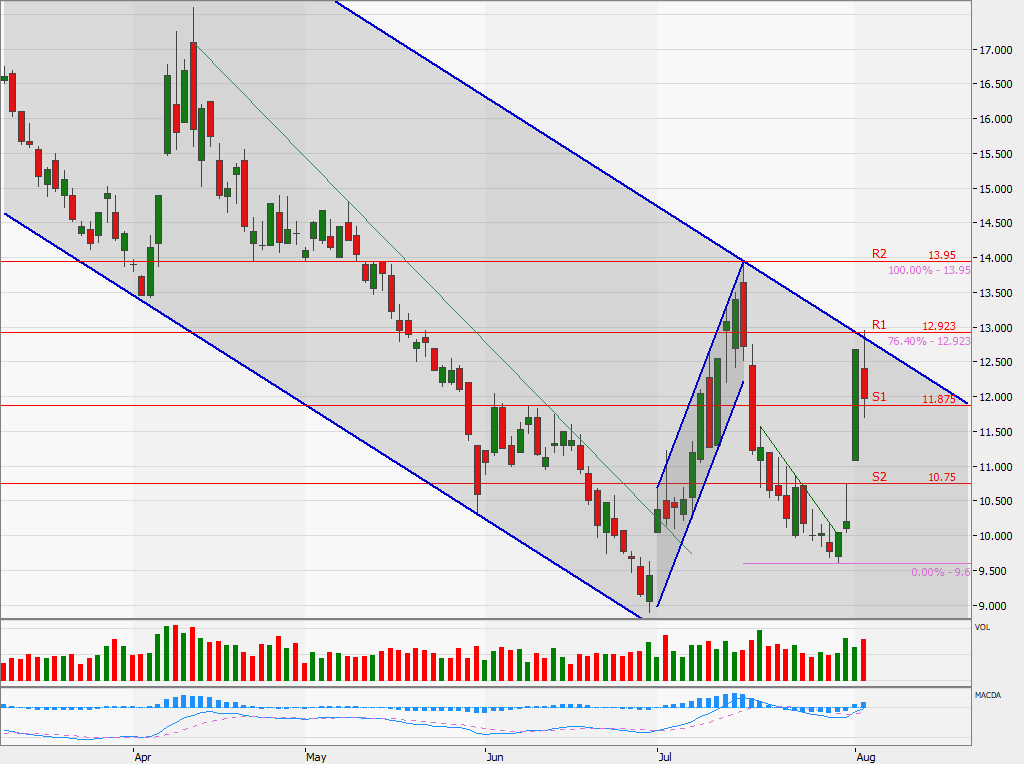
\includegraphics[scale=.30]{Image-2019-08-05-16-25-37} 
 
 \section{How can AI help ?}
Biggest difference AI can make is found out what works and what doesn't by Back testing every strategy and Indicator we can find out which of them works. It will make the method very efficient and people won't waste time on useless Indicators. \\
Second thing it can do is increase efficiency, We see a lot of patterns in charts and Also ignore a lot of patterns with naked eye there is always a chance of error but with help of AI we can pinpoint it to exact pattern and see if it has worked in past or not, And we can find out false signals too.
\\
Since there were a lot of naive traders trading with technical analysis so the professionals developed strategies to trade against them and it became a zero sum game, If retail traders will use those strategies too they will not be susceptible to huge losses.

\section{Future Of Trading }
Most of the hedge fund today use Fundamental Analysis (It uses various information about the company to determine it's stock performance) or Quantitative methods which is maths combined with Technical Analysis. However in recent times they have shifted towards using AI and Machine learning they developed many strategies using Arbitrage or Data to find profits. 
\\
Maybe with the help of AI we can prove Technical Analysis to be true Science or it may go other way and show us that it is utterly useless in both the cases it is good for financial markets and retail Traders.

\end{document}
